\section{Falcon工具的可视化}
\subsection{可视化的目标}
原始版的Falcon工具虽然可以具体定位到每一个数据访问模式的变量名和所在的语句,但由于结果只能以纯文字的格式显示,仍然不便于程序员迅速发现和定位错误。所以本文作者希望能够通过高亮显示的方式来突出包含错误模式的语句。同时希望将选择被测程序、插装、运行被测程序等一系列操作统一到一个图形化界面的工具里。
\subsection{可视化的实现}
\subsubsection{MVC设计模式}
MVC模式(Model-View-Controller)是软件工程中的一种软件架构模式。MVC是以模型(Model)、视图(View)和控制器(Controller)三个单词的首字母缩写命名。使用MVC模式可以减少代码之间的耦合。MVC模式的三个模块相互独立,改变其中一个不会影响其他两个,从而提高了应用程序的灵活性和可配置性。\par
模型用来封装应用程序的业务逻辑和基础数据。模型对外提供接口,可以被控制器和视图调用。视图是应用程序与用户的接口,作用是负责显示,即表达逻辑的内容。视图是模型的外观,可以访问模型的数据,但不能改变这些数据。视图只需要知道模型提供的接口,而不需要了解模型的内部逻辑。控制器是模型和视图之间的桥梁。控制器的作用是接受视图请求,并做出反应,执行相应的控制流,或者把响应结果返回到视图\cite{LiMVC}。\par
在Falcon可视化工具的实现过程中使用了MVC设计模式,这一部分的UML图如图\ref{pic:MVCUML}所示。
\begin{figure}[!ht]
  \centering
  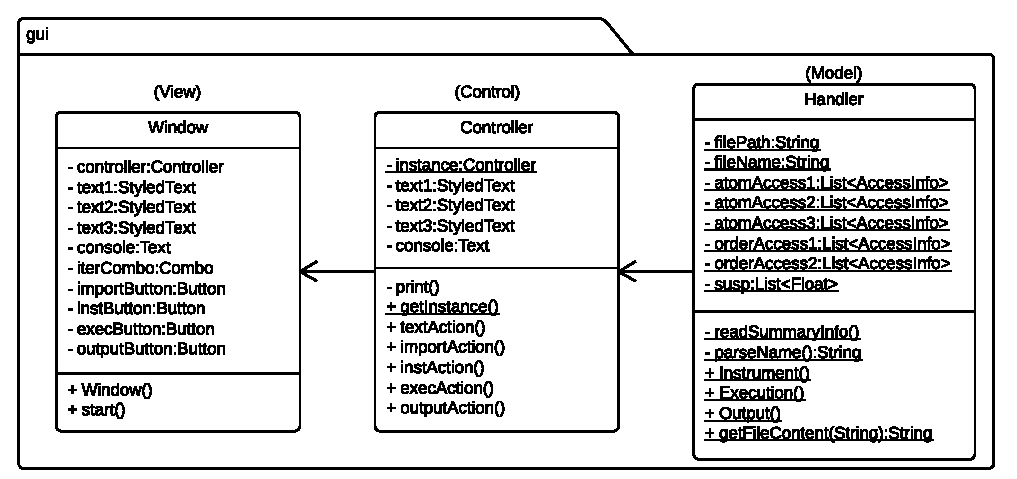
\includegraphics[width=\textwidth]{MVCUML.pdf}\\
  \caption{MVC设计模式的UML类图}\label{pic:MVCUML}
\end{figure}
\subsubsection{SWT框架}
SWT(Standard Widget Toolkit,标准部件工具包)是在Java平台下的一个图形化部件工具包。SWT最初由IBM公司主导开发,现在作为Eclipse集成开发环境的一部分由Eclipse基金会维护\cite{swt_wiki}。\par
和Java AWT、Java Swing等其它相比,SWT主要有以下优势:
\begin{enumerate}
  \item 界面与本地操作系统对应;
  \item 简单实用的API可以是开发人员快速上手;
  \item SWT应用程序运行速度快\cite{SWT}。
\end{enumerate}\par
在Falcon的可视化工具中,如何使含有错误的代码高亮显示是一个难点。在SWT中,提供了StyledText部件可以用来显示带有格式的文本,实现诸如加粗、背景色等显示效果。在窗口中添加StyledText对象,并调用\texttt{addLineBackgroundListener()}方法,实现LineBackgroundListener接口中的\texttt{lineGetBackground()}方法,即设定需要高亮显示的行数\textit{line}和背景的样式。当StyledText 对象中加入了文字之后,就可以触发LineBackgroundEvent,LineBackgroundListener监听到事件后,就把第\textit{line} 行按照之前的设置高亮显示出来。
\subsection{可视化的效果}
Falcon的可视化工具效果如截图\ref{Screen}所示。
\begin{figure}[!ht]
  \centering
  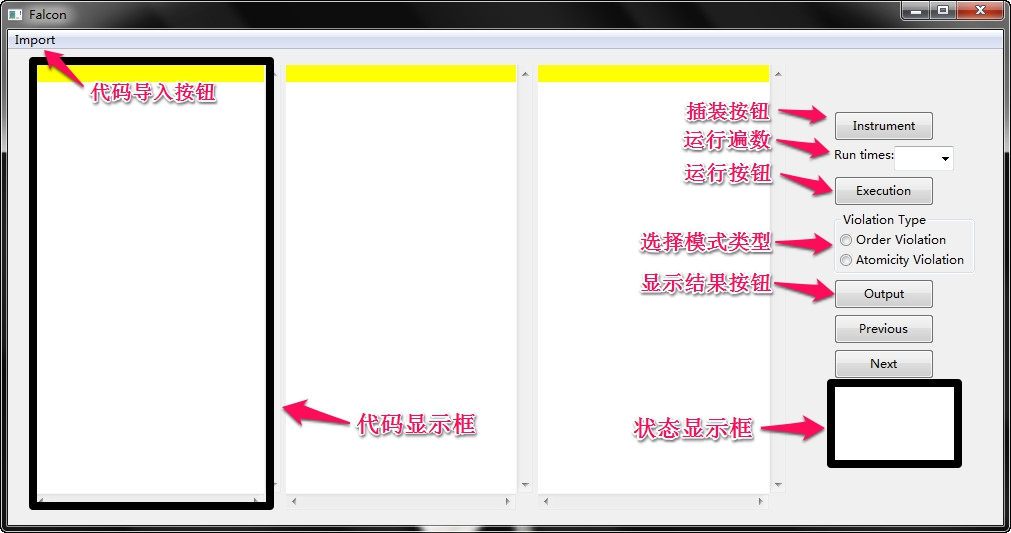
\includegraphics[width=.8\textwidth]{Screen.jpg}\\
  \caption{Falcon的可视化工具}\label{Screen}
\end{figure}
在使用时,首先需要导入被测程序。点击菜单栏上的Import按钮,选择被测程序中包含有主方法的类。如图\ref{ChooseFile}所示。
\begin{figure}[!ht]
  \centering
  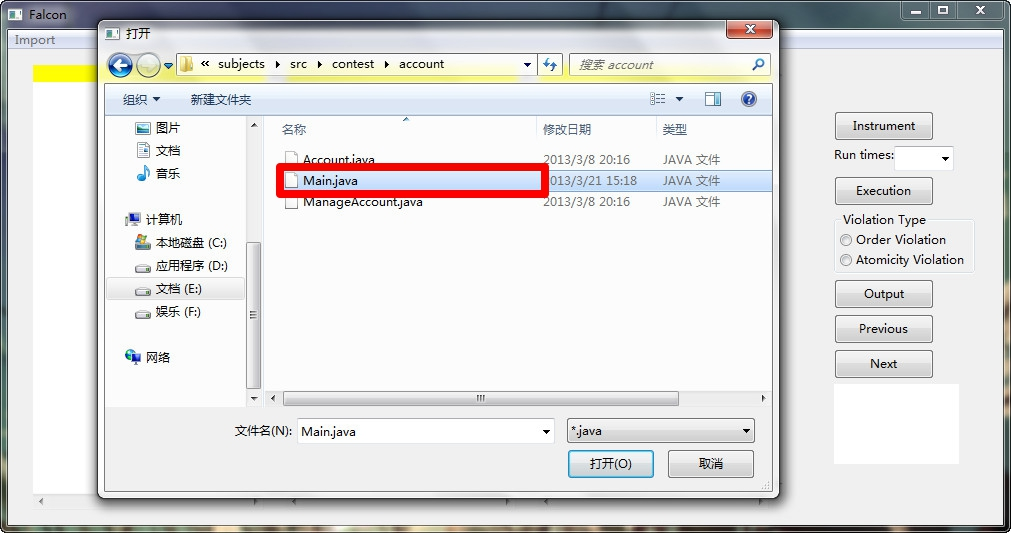
\includegraphics[width=.8\textwidth]{ChooseFile.jpg}\\
  \caption{选择被测程序中包含有主方法的类}\label{ChooseFile}
\end{figure}
点击Instrument按钮可以进行插装。在Run Times里可以选择被测程序执行的次数,然后点击Execution按钮可以运行被测程序。点击Output按钮之后,文本框中会出现被测程序的代码。包含有错误的访问模式所在的代码行被黄色高亮显示。在右下角的显示框内,会显示这个访问模式的具体信息,包括可疑度,模式类型,变量名等。
\begin{figure}[!ht]
  \centering
  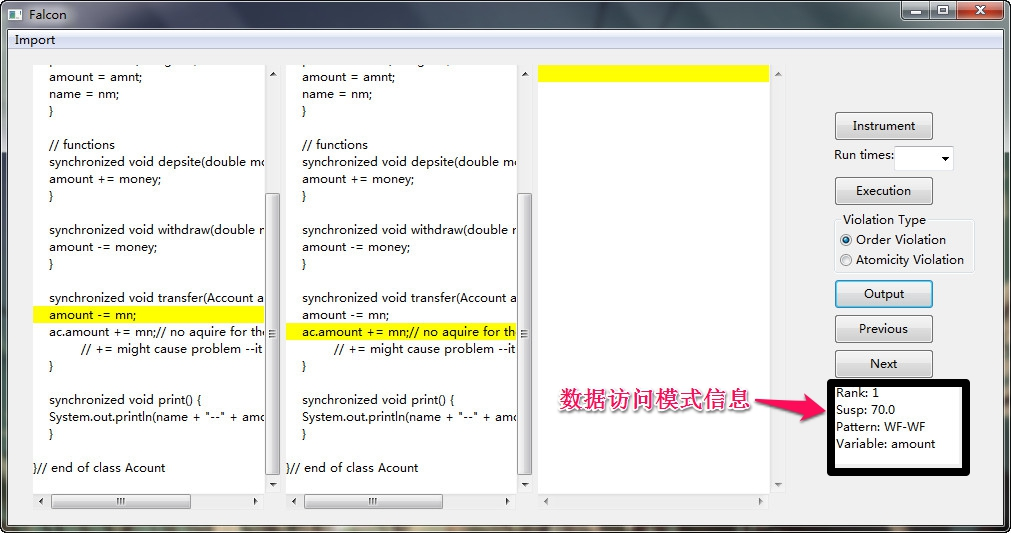
\includegraphics[width=.8\textwidth]{order.jpg}\\
  \caption{顺序性破坏显示效果}
\end{figure}
点击Next按钮则可以显示后一个错误的模式,点击Previous按钮可以显示前一个错误的模式。
\begin{figure}[!ht]
  \centering
  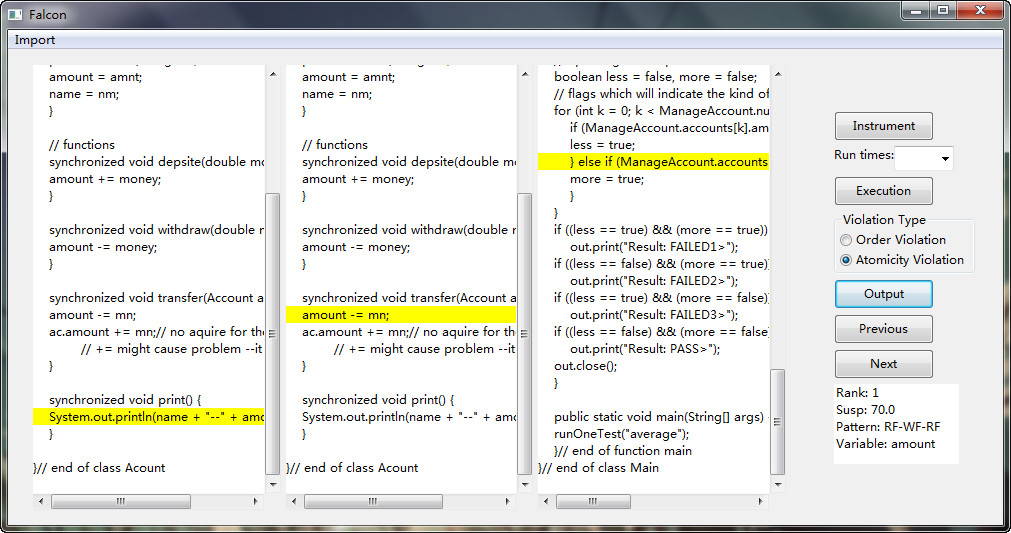
\includegraphics[width=.8\textwidth]{atom.jpg}\\
  \caption{原子性破坏显示效果}
\end{figure}
\subsection{与CORE的对比}
在Sangmin Park提出了Falcon的方法之后,乔治亚理工学院的两个研究生,Deepal Jayasinghe和Pengcheng Xiong,也尝试将Falcon扩展成为可视化工具。他们最终开发出了名为CORE的可视化并发错误定位工具\cite{CORE}。\par
CORE可以提供两个层次的视图来显示结果。如图\ref{pic:core}所示,低层次的视图用来显示数据访问模式中变量和方法的详细信息。高层次的视图用来显示模式的的可疑度等统计信息。此外,CORE提供了更为丰富的信息,包括插装信息、方法调用序列等。
\begin{figure}[!ht]
  \centering
  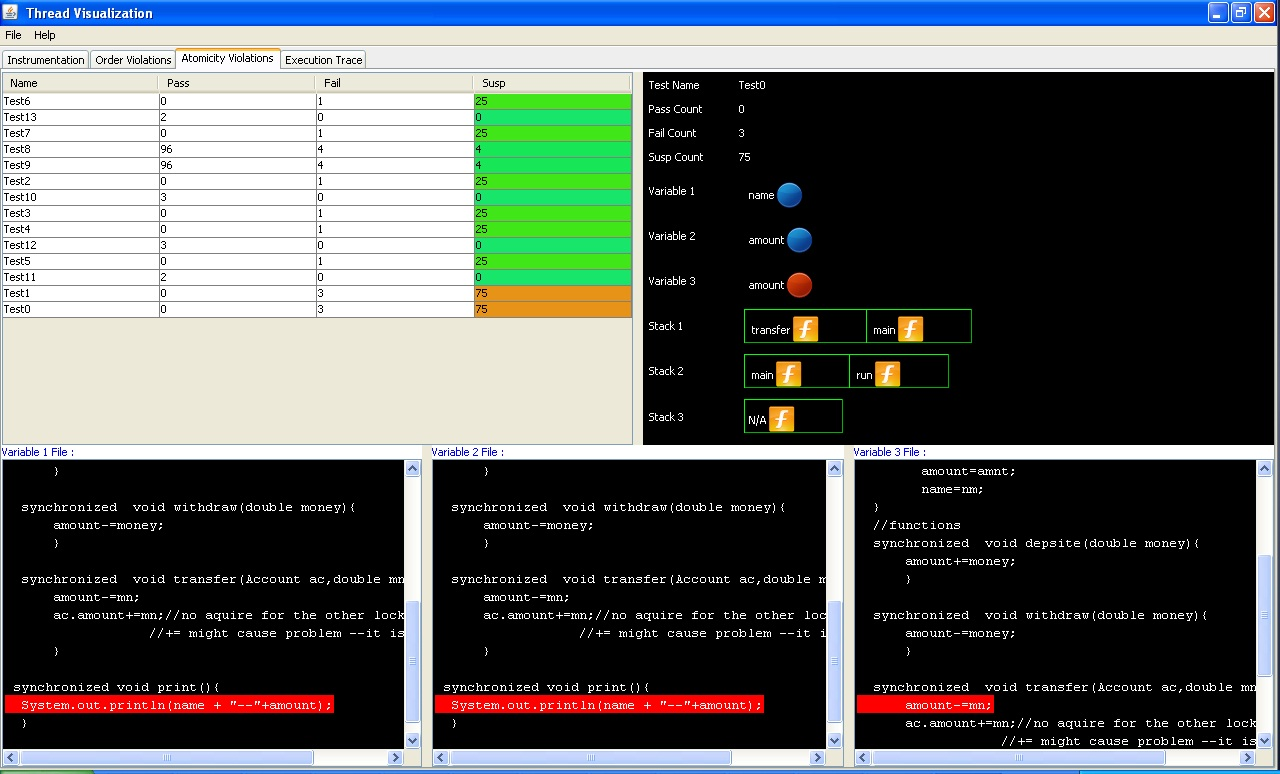
\includegraphics[width=.8\textwidth]{CORE.jpg}\\
  \caption{CORE的显示效果}\label{pic:core}
\end{figure}
与CORE相比,本文中的可视化工具有如下特点:
\begin{enumerate}
  \item 界面更加简洁;
  \item 操作更加简单;
  \item 将插装、运行被测程序这两个步骤集中到可视化工具当中。
\end{enumerate}
